\documentclass[10pt, conference, compsocconf]{IEEEtran}

\hyphenation{data-bases}

\newcommand{\TITLE}{Peer comparison of XSEDE and NCAR publication data}
\newcommand{\AUTHOR}{Gregor von Laszewski, Fugang Wang}

%%%%%%%%%%%%%%%%%%%%%%%%%%%%%%%%%%%%%%%%%%%%%%%%%%%%%%%%%%%%%%
% LATEX DEFINITIONS 
%%%%%%%%%%%%%%%%%%%%%%%%%%%%%%%%%%%%%%%%%%%%%%%%%%%%%%%%%%%%%%

\usepackage{cite}
\usepackage{float}
\usepackage{comment}
\usepackage{hyperref} 
\usepackage{array} 
\usepackage{graphicx} 
\usepackage{booktabs} 
% \usepackage{pifont} 
% \usepackage{todonotes} 
% \usepackage{rotating} 
% \usepackage{color} 
\usepackage{caption}
%\captionsetup{font={scriptsize}}

\newcommand*\rot{\rotatebox{90}} 
 
\newcommand{\FILE}[1]{\todo[color=green!40]{#1}} 
 

%
% more floats on one page
%
\renewcommand{\topfraction}{.85}
\renewcommand{\bottomfraction}{.7}
\renewcommand{\textfraction}{.15}
\renewcommand{\floatpagefraction}{.66}
\renewcommand{\dbltopfraction}{.66}
\renewcommand{\dblfloatpagefraction}{.66}
\setcounter{topnumber}{9}
\setcounter{bottomnumber}{9}
\setcounter{totalnumber}{20}
\setcounter{dbltopnumber}{9}

%%%%%%%%%%%%%%%%%%%%%%%%%%%%%%%%%%%%%%%%%%%%%%%%%%%%%%%%%%%%%%
% HYPERSETUP 
%%%%%%%%%%%%%%%%%%%%%%%%%%%%%%%%%%%%%%%%%%%%%%%%%%%%%%%%%%%%%%

\hypersetup{ 
    bookmarks=true,         % show bookmarks bar 
    unicode=false,          % non-Latin characters in Acrobat's bookmarks 
    pdftoolbar=true,        % show Acrobat's toolbar 
    pdfmenubar=true,        % show Acrobat's menu 
    pdffitwindow=false,     % window fit to page when opened 
    pdfstartview={FitH},    % fits the width of the page to the window 
    pdftitle={\TITLE},    % title 
    pdfauthor={\AUTHOR},     % author 
    pdfsubject={Subject},   % subject of the document 
    pdfcreator={Gregor von Laszewski, Fugang Wang},   % creator of the document 
    pdfproducer={}, % producer of the document 
    pdfkeywords={hindex} {metric}{XSEDE} {FutureGrid}, % list of keywords 
    pdfnewwindow=true,      % links in new window 
    colorlinks=false,       % false: boxed links; true: colored links 
    linkcolor=red,          % color of internal links (change box color with linkbordercolor) 
    citecolor=green,        % color of links to bibliography 
    filecolor=magenta,      % color of file links 
    urlcolor=cyan           % color of external links 
} 

\begin{document}

\begin{comment}
%\conferenceinfo{submitted to XSEDE}{'15,  July 26 - 30 2015, St. Louis, MO, USA}
\conferenceinfo{submitted to ...}{2015,USA}
\CopyrightYear{2015} 
\crdata{TBD...\$15.00.\\
http://dx.doi.org/TBD
} 
\end{comment}

\title{\TITLE\vspace{-12pt}}



\begin{comment}
\numberofauthors{3}  
\author{ 
\alignauthor 
Gregor von Laszewski\titlenote{Corresponding Author.}\\ \vspace{2pt}
Fugang Wang\\ \vspace{2pt}
Geoffrey C. Fox\\ \vspace{6pt}
       \affaddr{Indiana University}\\ 
       \affaddr{2719 10th Street}\\ 
       \affaddr{Bloomington, Indiana, U.S.A.}\\ 
\and  
\alignauthor  David L. Hart\\ \vspace{6pt}
       \affaddr{Computational and Information Systems Laboratory National Center for Atmospheric Research}\\
       \affaddr{P.O. Box 3000}\\
       \affaddr{Boulder CO 80307-3000}\\
\and
\alignauthor  
Thomas R. Furlani\\ \vspace{2pt}
Robert L. DeLeon\\ \vspace{2pt}
Steven M. Gallo\\ \vspace{6pt}
       \affaddr{Center for Computational Research}\\
       \affaddr{University at Buffalo, SUNY}\\ 
       \affaddr{701 Ellicott Street}\\ 
       \affaddr{Buffalo, New York, 14203}
}

\date{28 May 2014}
\end{comment}

\begin{comment}
\author{\IEEEauthorblockN{%
Gregor von Laszewski,
Fugang Wang,
Geoffrey C. Fox}
\IEEEauthorblockA{School of Informatics and Computing\\
Indiana University\\
Bloomington, Indiana, U.S.A.\\
laszewski@gmail.com}
\and
\IEEEauthorblockN{David L. Hart}
\IEEEauthorblockA{%
Computational and Information Systems Laboratory\\
NCAR\\
Boulder CO 80307-3000}
\and
\IEEEauthorblockN{Thomas R. Furlani,
Robert L. DeLeon,
Steven M. Gallo}
\IEEEauthorblockA{%
Center for Computational Research\\
University at Buffalo, SUNY\\ 
Buffalo, New York, 14203}
}
\end{comment}

\author{\IEEEauthorblockN{%
Gregor von Laszewski$^1$,
Fugang Wang$^1$,
Geoffrey C. Fox$^1$
David L. Hart$^2$\\
Thomas R. Furlani$^3$,
Robert L. DeLeon$^3$,
Steven M. Gallo$^3$}
\IEEEauthorblockA{%
$^1$School of Informatics and Computing, Indiana University, Bloomington, Indiana, U.S.A.\\
$^2$Computational and Information Systems Laboratory, NCAR, Boulder CO 80307-3000, U.S.A.\\
$^3$Center for Computational Research, University at Buffalo, SUNY, Buffalo, New York, 14203, U.S.A.\\
 laszewski@gmail.com}
}

\maketitle

\begin{abstract}

We present a framework that compares the publication impact based on a comprehensive peer analysis of papers produced by scientists using XSEDE and NCAR resources. The analysis is introducing a percentile ranking based approach of citations of the XSEDE and NCAR papers compared to peer publications in the same journal that do not use these resources.  This analysis is unique in that it evaluates the impact of the two facilities by comparing the reported publications from them to their peers from within the same journal issue. From this analysis, we can see that papers that utilize XSEDE and NCAR resources are cited statistically significantly more often.  Hence we find that reported publications indicate that XSEDE and NCAR resources exert a strong positive impact on scientific research.

\end{abstract}

\begin{IEEEkeywords}
Metrics; publications
\end{IEEEkeywords}


\begin{comment}
\vspace{-6pt}

\category{H.4}{Information Systems Applications}{Miscellaneous}
\category{D.2.8}{Software Engineering}{Metrics}[complexity measures,
performance measures]

\terms{Theory, Measurement}

\keywords{Scientific impact, bibliometric, h-index, Technology Audit
  Service, XDMoD, XSEDE}
\end{comment}

\section{Introduction} 


We analyze the scientific impact on {\em scientific advancements enabled by enhanced cyberinfrastructure} for XSEDE and NCAR resources. We extend our previous work \cite{las14impact} by comparing publication impact based on a comprehensive peer analysis carried out on papers produced by scientists using XSEDE and National Center for Atmospheric Research (NCAR) resources \cite{las15cluster-long,las15xsede}. The analysis is based on a percentile ranking of citations of the papers derived from a comparison to peer publications in the same journal not using the resources. The result shows that papers that utilize XSEDE and NCAR resources tend to be cited more often than their peers are cited. We leverage for this work the data collection and processing architecture described in \cite{las14impact,las15cluster-long}. To conduct the analysis, the general workflow includes obtaining the publication data for each XSEDE user, and then retrieving the citation data for each publication. Hence, the data is originally collected on a per-user and per-publication basis. As part of processing, the data are aggregated based on organization, XSEDE project/account, and FOS.  By correlating the publication data with XSEDE usage and allocation data (for example the allocation amounts awarded by XSEDE), our intention is to determine if the analysis reveals patterns and trends in how XSEDE impacts the sciences and possibly to help better measure the return on investment (ROI) for NSF. Naturally, the same is applied to the NCAR data to demonstrate the generality of our methods.

\section{Metric for Journal Publication-based Peer Comparison} \label{S:metric}

We compare XSEDE and NCAR publications with their peers (more than one million publication) by looking at the citation count and relative ranking through the following process: 
(1) Identify publication venues of the reported XSEDE or NCAR publications;
(2) Retrieve all publication data from those venues during the same time period;
(3) Identify the peers comparison groups (all publications in same journal issues);
(4) Calculate ranking scores of XSEDE/NCAR publications and their peers; and
(5) Use the raw ranking scores to derive comparison metrics at different aggregation level (e.g. journal, Field of Study).

We define a \emph{performance score} based on weighted sum of the percentages of publications falling into each quarter by percentile ranking:

\[	S = 1*P_{Q_1} + 0.5*P_{Q_2}+ (-0.5)*P_{Q_3} + (-1)*P_{Q_4} \]

where, $P_{Q_i}$ is the percentage of publications falling into the top $i$-th quarter, $P_{Q_i} \in [0,1]$ and $\sum_{i} {P_{Q_i}} = 1$ for one aggregated subject (a journal or one FOS). As $S \in [-1, 1]$ and the possible values are symmetric, a positive value implies more publications appear in the upper half in ranking and negative means more in the lower half.

\section{XSEDE Peer Data Analysis}
\label{S:xsede}

We apply the procedure and then aggregate the raw percentile ranking scores at journal level, and calculate the average and median percentile ranking for each journal, as well as the resulting \emph{performance score}. We include only those journals with at least ten publications so the results has a higher statistical relevance. Table \ref{T:groups_stats} compares the average and median rankings and citations received. The t-test shows that XSEDE publications are statistically higher ranking and have a higher  mean citation rate than the non-XSEDE peer group.

\begin{table}[h!]
\caption{Basic statistics of XSEDE publications group and peers group}
\label{T:groups_stats}
\centering
\begin{small}
\begin{tabular}{lrrrrrr}
 & Number of & \multicolumn{2}{ c }{Rank} & \multicolumn{2}{ c }{Citations}  \\
 &  Publications & Average & Median & Average & Median \\
\hline
  XD     & 2349	        & 61	& 65	& 26	& 11 \\
Peers & 168422	& 49	& 48	& 13	& 5 \\
\end{tabular}
\end{small}
\end{table}

\begin{enumerate}
\item T-test for ranking (Welch Two sample t-test)
\begin{enumerate}
\item T=21.4134, df=2412.99, p-value$<$2.2e-16
\item 95\% confidence interval: $[10.80, 12.98]$
\end{enumerate}
\item T-test for citation count:
\begin{enumerate}
\item T=7.057, df=2358.929, p-value=2.228e-12
\item 95\% confidence interval: $[9.40, 16.63]$
\end{enumerate}
\end{enumerate}



\begin{figure}[t!]
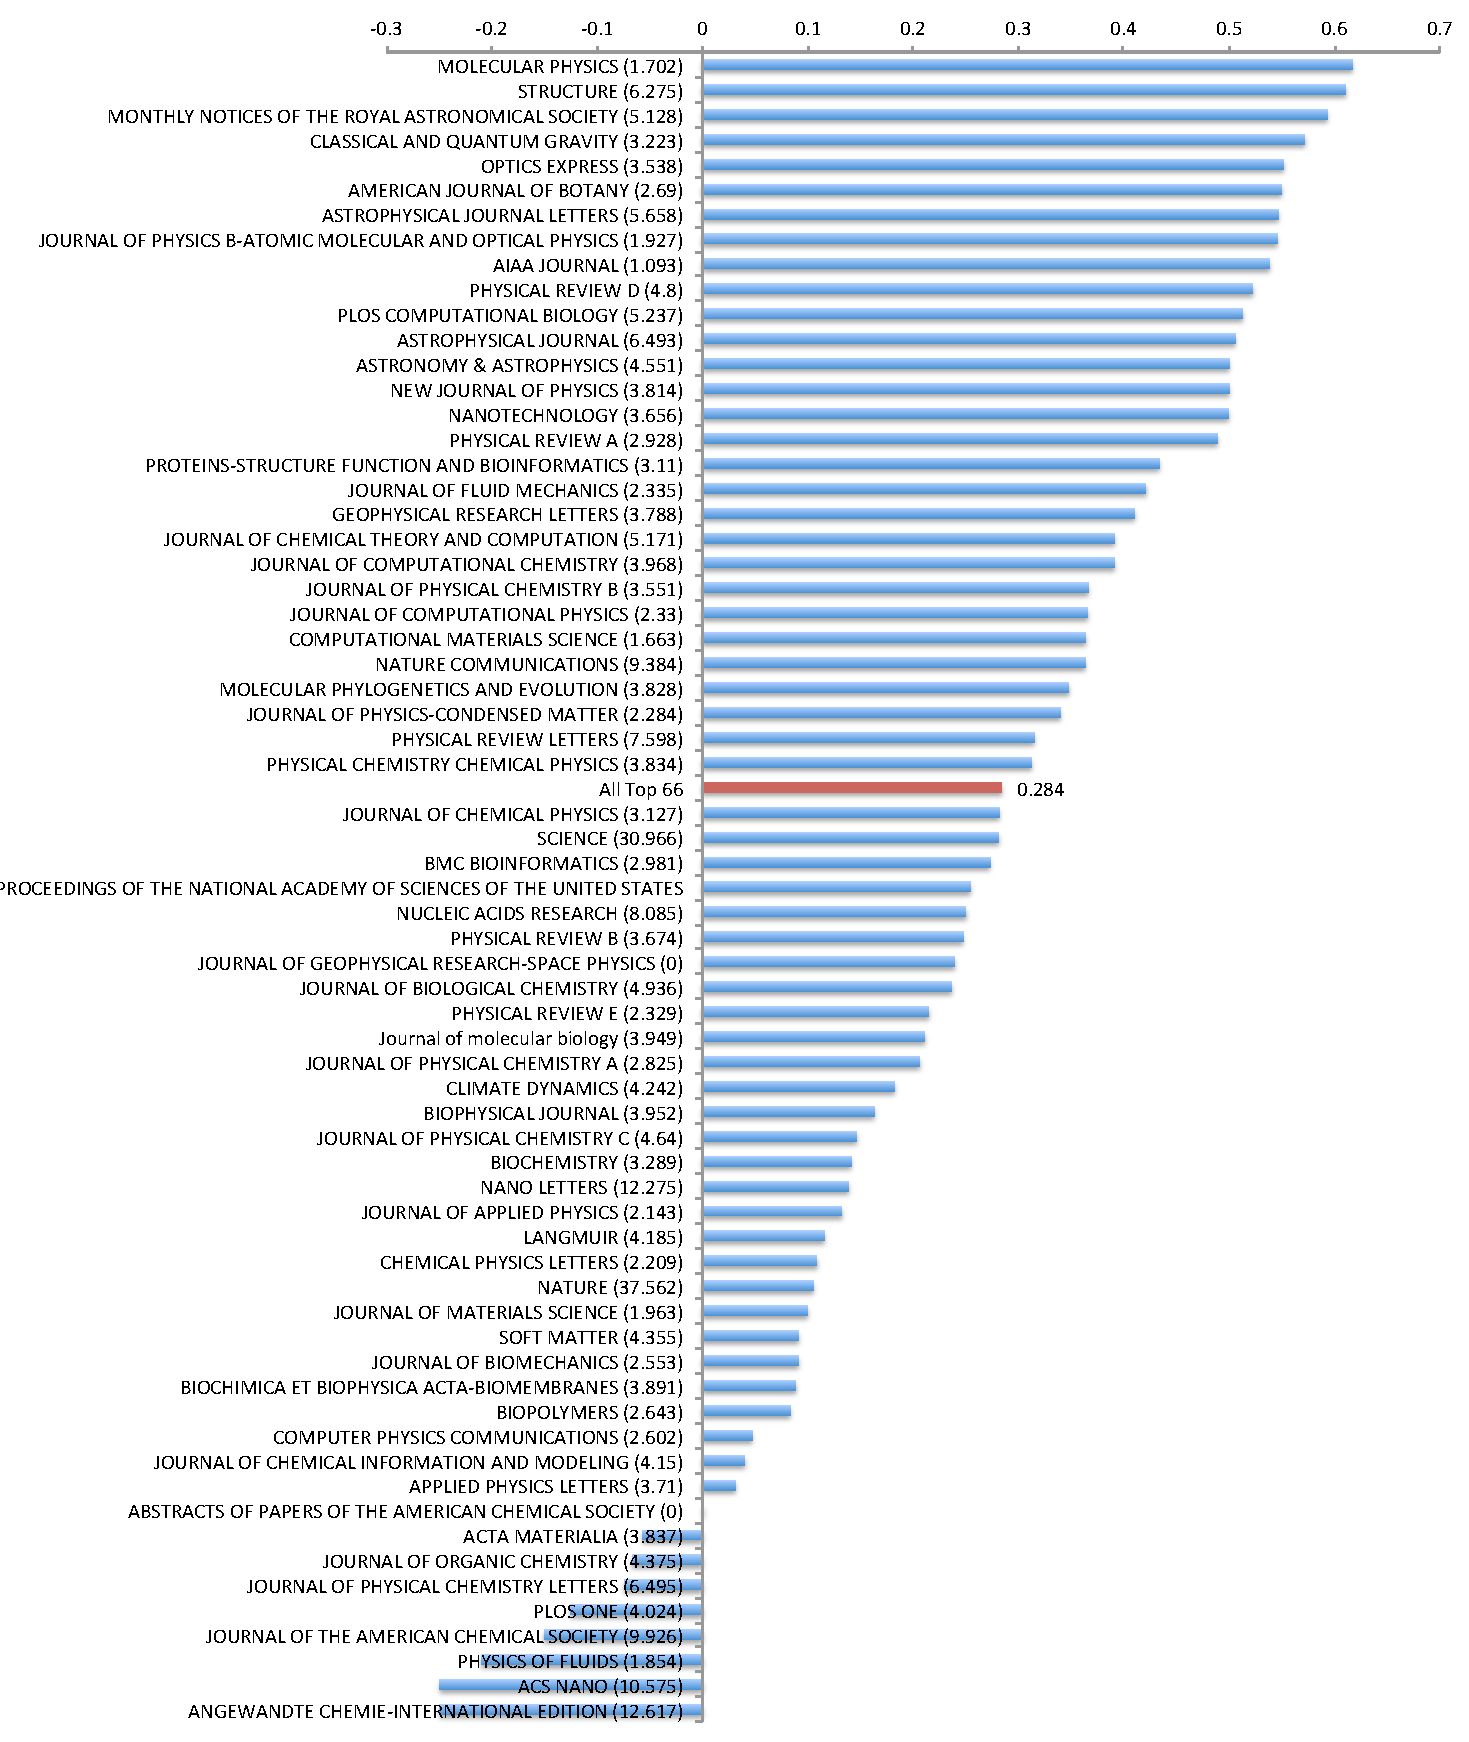
\includegraphics[width=.9\columnwidth]{images-new/xsede-journal-score.pdf} 
\vspace{-6pt}
\caption{The score of our peer comparison metric for XSEDE publications by journal.}\label{F:xsede-score}

%  \centering 
%    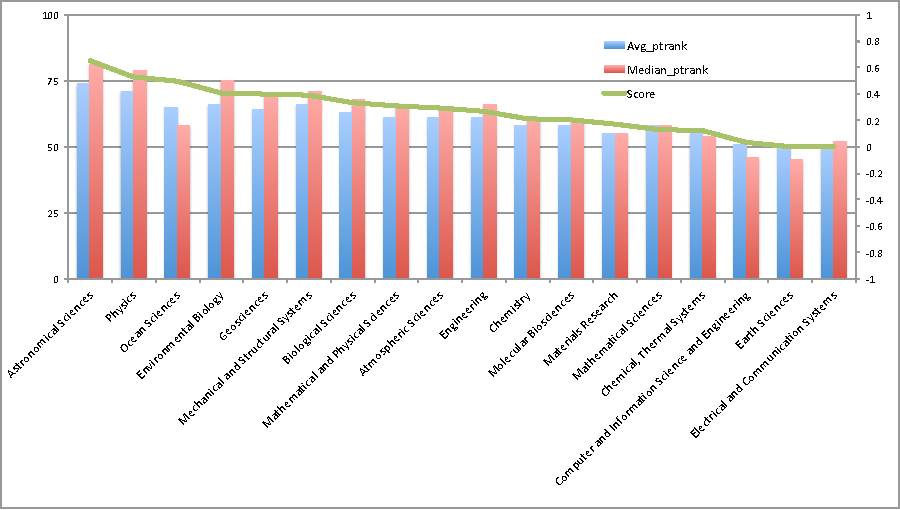
\includegraphics[width=1.0\columnwidth]{images-new/b.pdf} 
%\vspace{-18pt}
%  \caption{Peer comparison based on Parent Field of Science from the original analysis of XSEDE data.}\label{F:xsede-stacked-b} 

  \centering 
    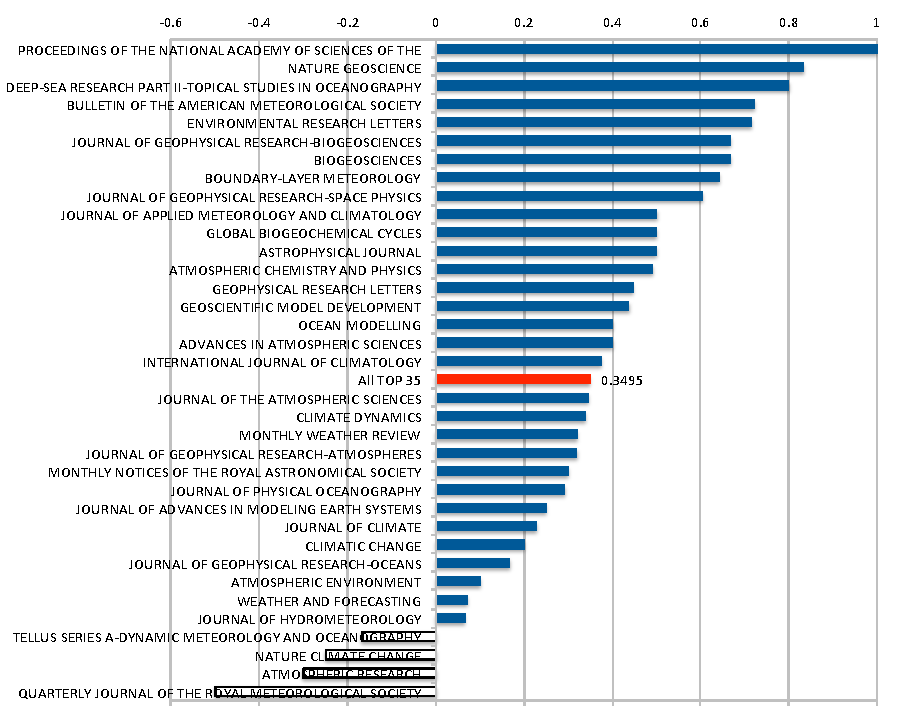
\includegraphics[width=1.0\columnwidth]{images-new/ncar-c.pdf} 
\vspace{-18pt}
  \caption{Peer comparison based on Parent Field of Science from the original analysis of NCAR data.}\label{F:ncar-score}
\end{figure} 







\begin{comment}

    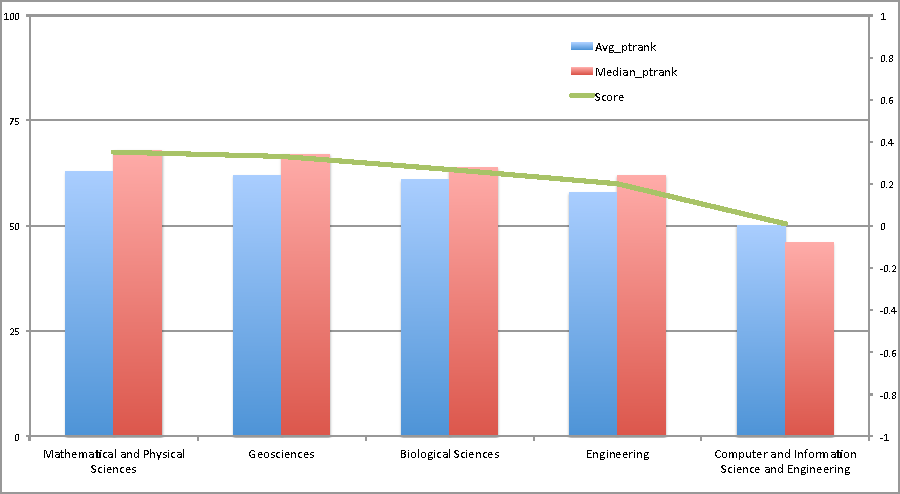
\includegraphics[width=1.0\columnwidth]{images-new/c.pdf} 
  \caption{Peers comparison based on the topmost Field of Science category as defined by NSF.}\label{F:xsede-top-c} 

\hfill



\begin{figure*}[htb!] 
  \centering 
    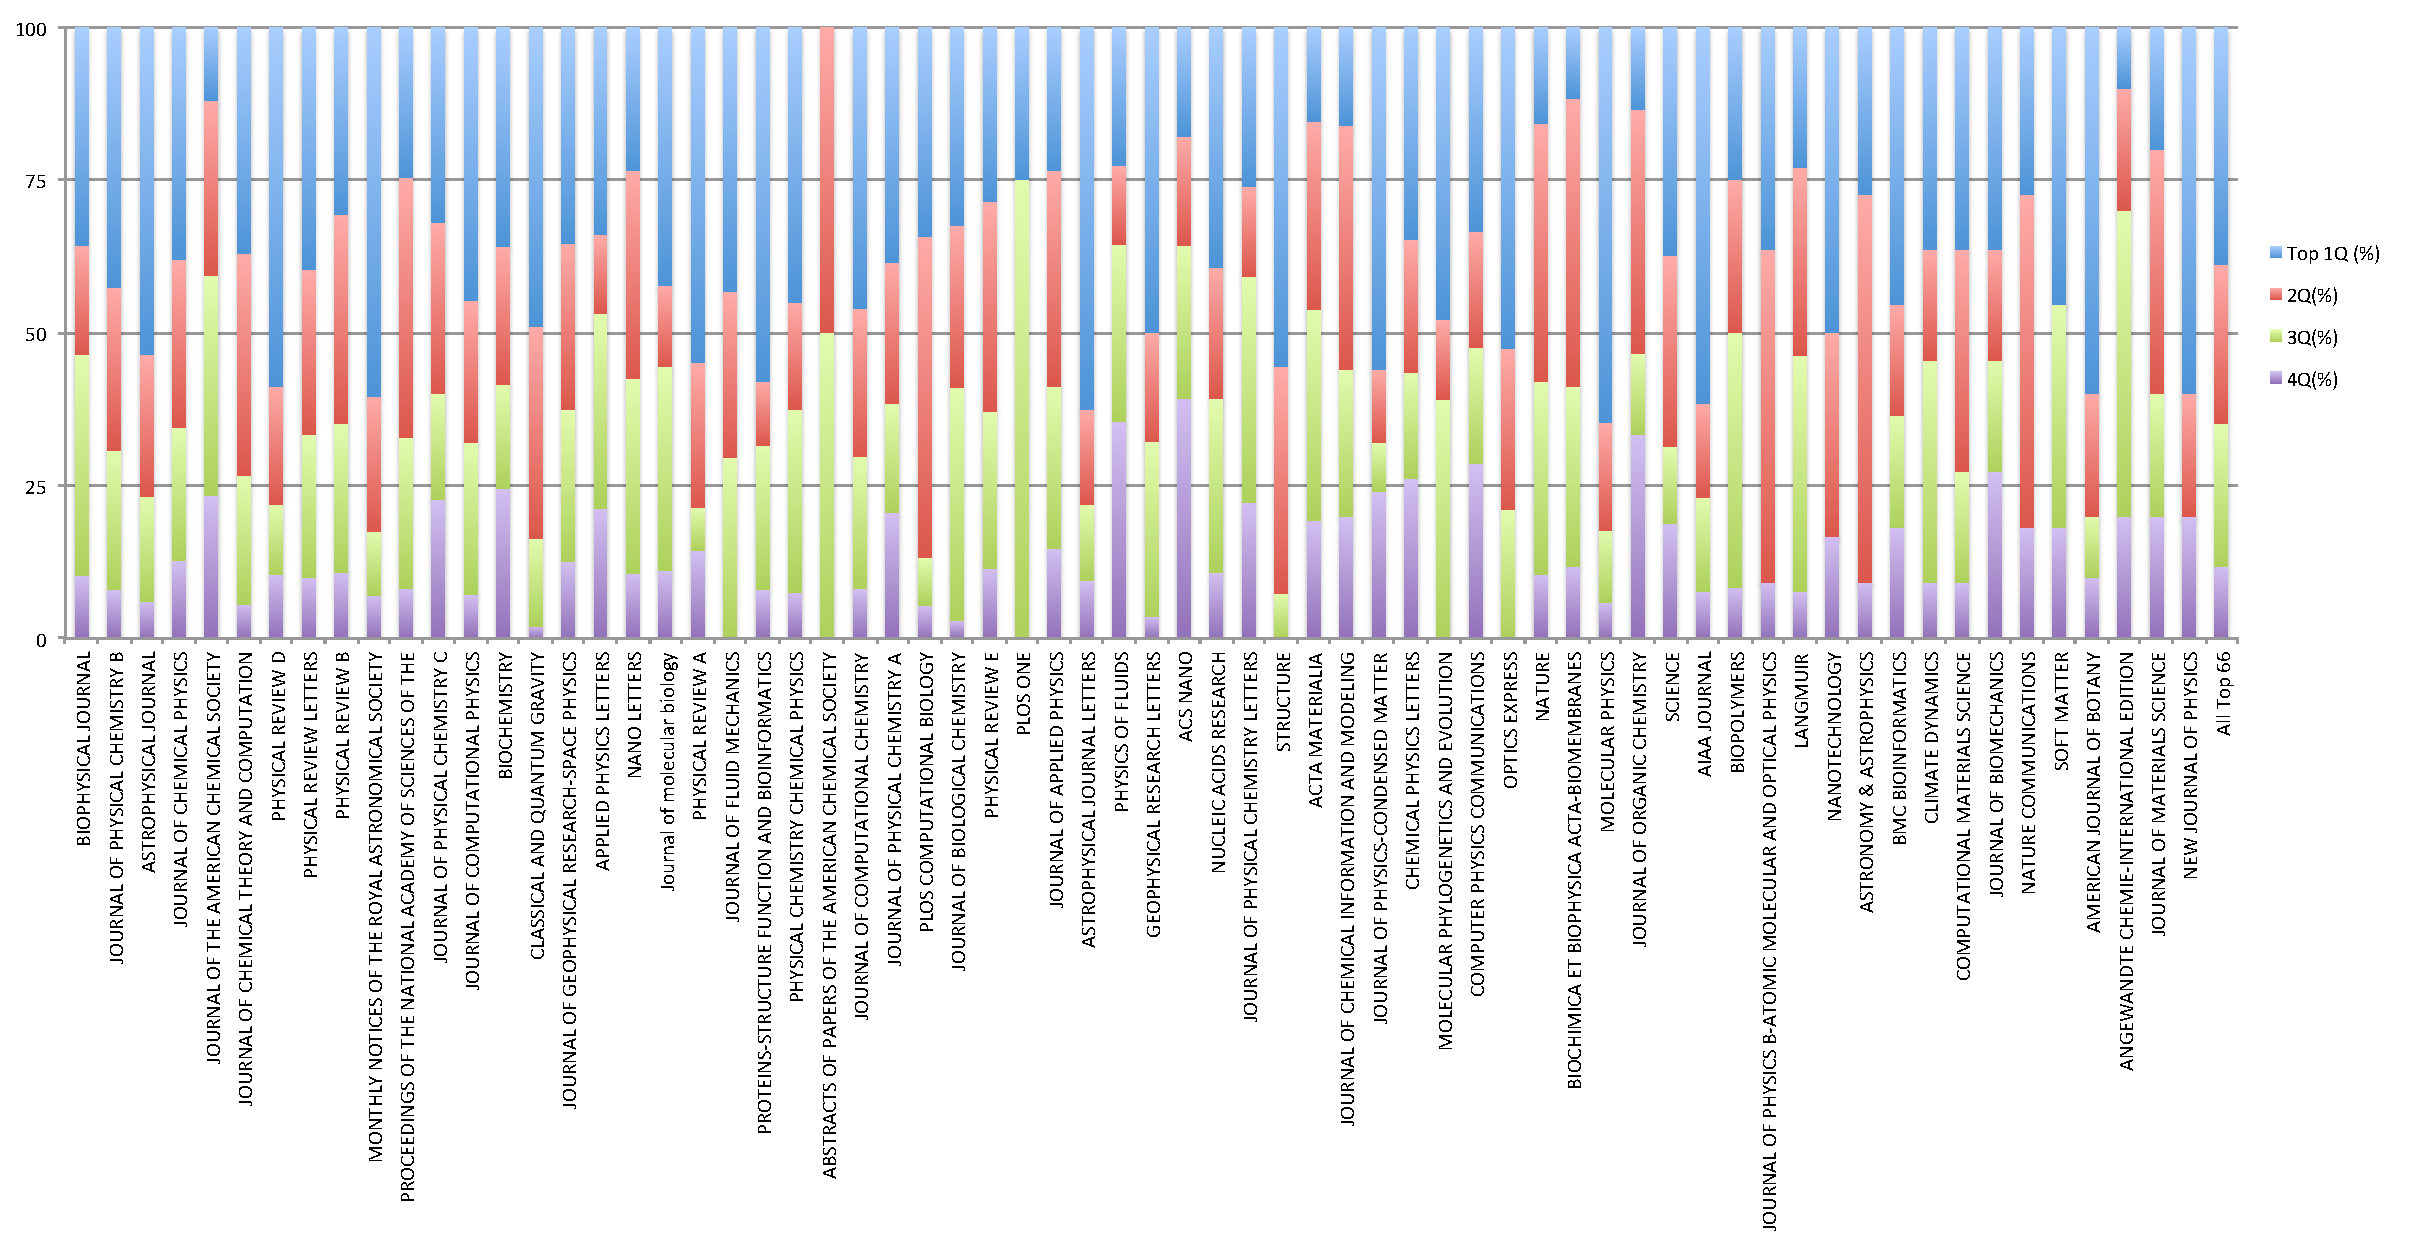
\includegraphics[width=1.0\textwidth]{images-new/xsede-journal-stacked.pdf} 
  \caption{Percentile ranking by journal in a stacked barchart of XSEDE publications.}\label{F:xsede-stacked} 
\end{figure*}

\bigskip

\end{comment}

we included the performance scores of the top 66 journals in which 10 or more XSEDE publications published (see Figure \ref{F:xsede-score}) and find that the overal score metric for all the involved journals is positive with a value of 0.284. This implies that researches benefit from use of XSEDE resources as the resulting publications tend to be cited more than their peers from the same journal.

When aggregating the individual results on the Field of Science (FOS) categories we observe \cite{las15cluster-long}  similar results as publications from most FOS perform better than their peers, while certain FOS such as Astronomy and physics benefit most from using XSEDE. Fields that perform not as good include Experimental and Theoretical Geochemistry, Geometric Analysis and Mechanical and Structural systems as they are typically not dependent on computational resources.

\section{NCAR Peer Data Analysis}\label{S:ncar}

\begin{comment}
  \centering 
    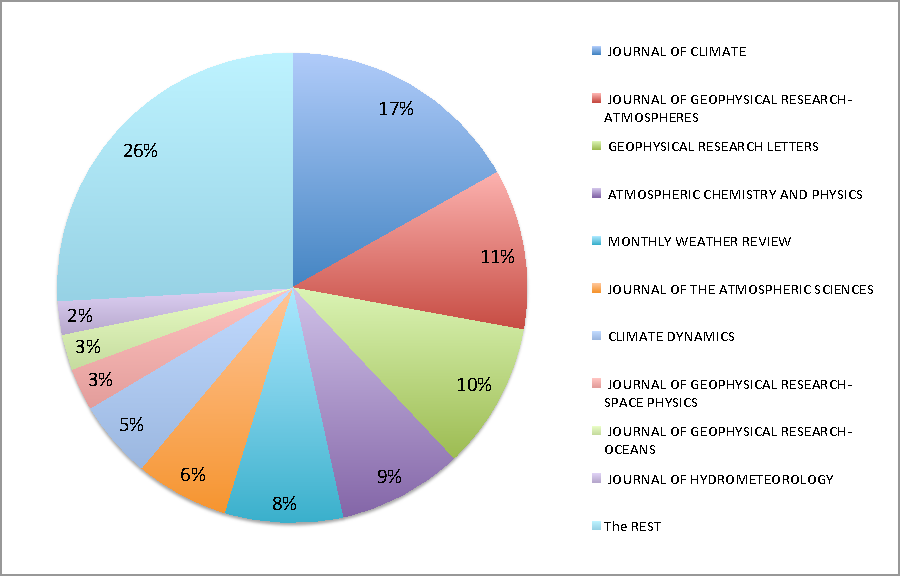
\includegraphics[width=0.75\columnwidth]{images-new/ncar-a.pdf} 
  \caption{Distribution of the top most journals by publication count.}\label{F:ncar-distribution} 

  \centering 
    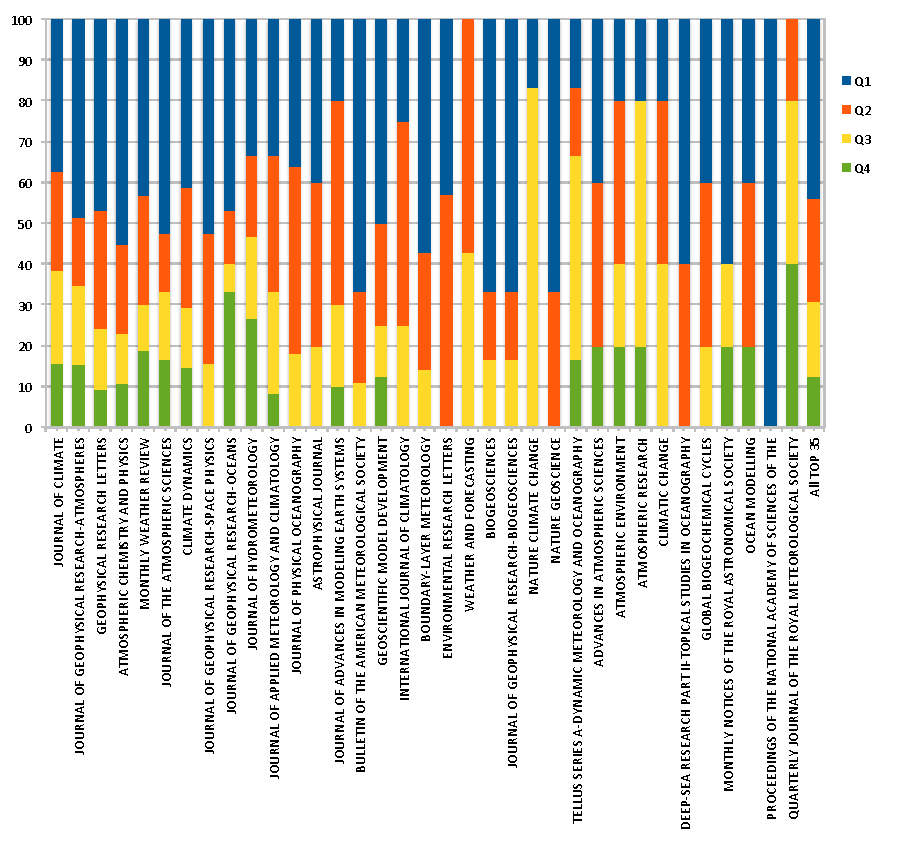
\includegraphics[width=1.0\columnwidth]{images-new/ncar-b.pdf} 
  \caption{Percentile ranging by FOS in a stacked barchart of NCAR publications.}\label{F:ncar-stacked-b} 
\end{comment}

We replicated the analysis with NCAR publication data of 900 records. Because the NCAR data set is smaller than the one from XSEDE, instead of looking at all journals that have at least ten publications, we reduced the value to five. This will give a large enough journal number to conduct our analysis. The \emph{performance score} as defined earlier is presented as in Figure \ref{F:ncar-score}. We observe a positive value of about 0.35 indicating the better performance than the peers'.

\section{Conclusion} \label{S:conclusion}

The NCAR score is slightly higher than that of XSEDE as XSEDE has a wider range of FOS. Computational intense disciplines such as atmospheric sciences result in the highest score values using the resources. For both XSEDE and NCAR publications, the impact metric measured by a performance score (defined based on percentile ranking) is positive and higher than their peers that have not used such resources.

%%%%%%%%%%%%%%%%%%%%%%%%%%%%%%%%%%%%%%%%%%%%%%%%%%%%%%%%%%%%%%%%%%%%%% 
% Acknowledgment 
%%%%%%%%%%%%%%%%%%%%%%%%%%%%%%%%%%%%%%%%%%%%%%%%%%%%%%%%%%%%%%%%%%%%%% 

\section*{Acknowledgments}

Supported by NSF \#1445806 influenced by 0910812.
 

%\bibliographystyle{IEEEtranS}
%\bibliographystyle{abbrvurl} 
\bibliographystyle{IEEEtran}
\bibliography{% 
vonlaszewski}



\end{document}

%%%%%%%%%%%%%%%%%%%%%%%%%%%%%%%%%%%%%%%%%%%%%%%%%%%%%%%%%%%%%%%%%%%%%%
%%%%%%%%%%%%%%%%%%%%%%%%%%%%%%%%%%%%%%%%%%%%%%%%%%%%%%%%%%%%%%%%%%%%%%
%%%%%%%%%%%%%%%%%%%%%%%%%%%%%%%%%%%%%%%%%%%%%%%%%%%%%%%%%%%%%%%%%%%%%%